% !TeX root = ../main/main.tex
\documentclass[../main/main.tex]{subfiles}

\begin{document}
\espacio

  En este capítulo se muestra en detalle la problemática de la investigación, la justificación del problema con una visión desde el paradigma tecnológico, así como los alcances y límites de la investigación.

  \section{Planteamiento del problema}

  En una computadora, al ejecutar acciones dentro de una aplicación se generan tareas, las tareas son divididas en procesos que la CPU\footnote{Central Processing Unit (Unidad Central de Procesamiento)} delega a sus diferentes núcleos físicos (en caso de contener más de uno), cada proceso genera hilos que los procesadores lógicos ejecutan para coverger en el resultado del proceso maestro. Estos trabajos son realizados a una frecuencia única en todos los núcleos de la CPU, esta frecuencia es llamada comúnmente velocidad del procesador.

  En la actualidad las CPUs cuentan con memorias cache de nivel 1 para datos e instrucciones, nivel 2 para almacenamiento efímero, y nivel 3 también conocido como LLC\footnote{Last Level Cache (Memoria Compartida de Último Nivel)} para datos compartidos entre los núcleos; el número indica la distancia del bus entre el procesador y cada nivel de memoria cache, a mayor distancia mayor número. Sin embargo, estas memorias son del orden de los Kilobytes hasta los Megabytes, tal es el caso, que estas memorias no se alejan de un máximo de 2MB, por tal motivo surge la necesidad de un dispositivo que incremente la capacidad de almacenamiento efímero. Aquí es donde entra en acción la memoria RAM\footnote{Random Access Memory (Memoria de Acceso Aleatorio)}, esta memoria sirve para almacenar datos que no se almacenan en un medio rígido como el disco duro pero que llega a pesar mas de lo que pueden albergar las memorias cache del CPU.

  \begin{figure}[ht]
    \centering
    \caption{Conexión de entre CPU, memorias cache y memoria RAM}
    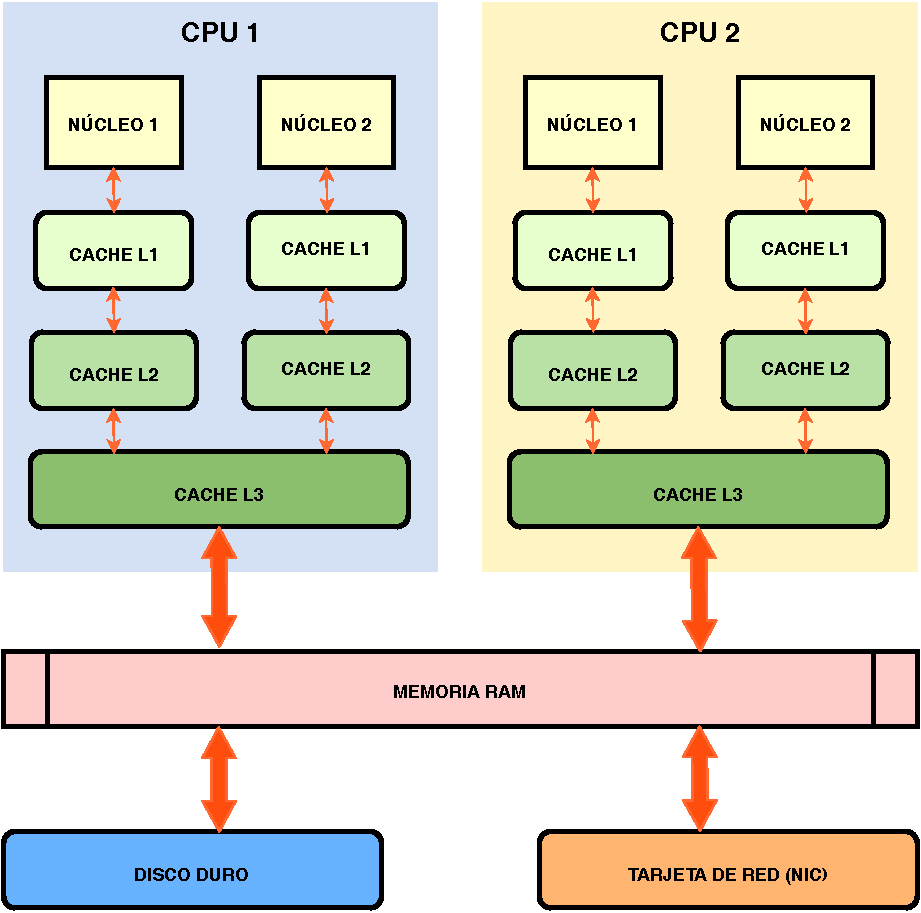
\includegraphics[width=10cm, keepaspectratio]{problema/cpu_cache_ram.pdf}
    \caption*{\textbf{Fuente:} Elaboración propia}
    \label{fig:cpu_cache_ram}
  \end{figure}

  La memoria RAM, al igual que el CPU, es regida por una frecuencia de trabajo que debe ser igual o menor que la frecuencia del CPU, como se observa en la Figura \ref{fig:cpu_cache_ram}, la distancia del bus entre los núcleos y ésta memoria es mayor que la distancia hacia las memorias cache, por tal razón la velocidad de transferencia de datos entre la CPU y ésta memoria es menor que la velocidad de las memorias cache de nivel 1, 2 y 3, tal como se explica en \cite[p.~126]{book:computer_architecture_stallings}.

  Sumando la velocidad de la CPU y la de la memoria RAM, se obtiene un resultado que conforma la mayor parte de la velocidad de una computadora. Los scripts de javascript que se ejecutan en los navegadores web hacen uso de estos dos elementos de una computadora. Por lo general los antivirus no realizan un monitoreo de las peticiones que se ejecutan desde javascript y los firewalls, tanto personales como de red, no restringen el tráfico a menos que exista una regla que lo especifique.

  Aprovechando esta situación, los gusanos que se introducen en el código javascript pueden utilizar un porcentaje del procesamiento de una computadora y tras obtener el resultado que buscaban, enviarlo a un servidor remoto. Este es un tipo de ataque conocido como ataque ``zombie'' pero en el caso de minería de criptomonedas no se intenta denegar ningún servicio, sino robar el procesamiento de los equipos clientes para generar hashes útiles en para la minería.

  El problema surge cuando el rendimiento de los equipos clientes se ve disminuido, cuestión que genera molestia en los clientes al utilizar el servicio infectado afectando así a la imagen del producto o de la empresa que brinda dicho servicio, reduciendo de esta manera el número de clientes.

  Por otra parte, desde el enfoque de una empresa, cuando los empleados hacen uso de un servicio infectado con este tipo de gusanos generan un ticket de soporte técnico y en muchos casos el personal que brinda soporte técnico no llega a detectar la falla y brinda como única solución la de incrementar las características del equipo, cuestión que representa un gasto por el tiempo en el que el personal de soporte técnico llega a ``solucionar'' el problema y el hardware adquirido para ello, sin darse cuenta de que el problema persiste y solo se ha dado paso a que la infección persista por mayor tiempo.

  \section{Justificación tecnológica}

  Por la popularidad que ha adquirido el entorno de virtualización de contenedores Docker, conjuntamente con la popularidad de los servicios en la nube como AWS de Amazon, Google Cloud o Microsoft Azure, se deben definir tecnologías y procesos para garantizar la seguridad en entornos virtualizados y sumarlas a los recursos de seguridad existentes para redes y aplicaciones específicas.

  Para el caso específico de Graboid, el gusano utilizado para minería de criptomonedas desde imágenes de Docker; dada la dificultad de detección de este tipo de gusano y su reciente identificación, es indispensable exponer la mayor información posible acerca del proceso de infección y el flujo que inicia con el montaje de un sevicio infectado hasta el proceso que se ejecuta en los clientes a fin de evitar y/o detectar, de manera temprana, este tipo de infecciones y no recaer en los gastos consecuentes mencionados anteriormente.

  \section{Alcances y límites}

  El objeto de análisis es el gusano Graboid, este gusano fue descubierto el 16 de Octubre de 2019 por los investigadores de la Unidad 42 de Paloalto Networks de acuerdo al resumen ejecutivo publicado por \cite{web:graboid_paloalto}.

  Al momento del desarrollo del presente análisis, una gran parte de las imágenes infectadas con el gusano Graboid fuerón eliminadas del repositorio oficial de \href{https://hub.docker.com/}{Docker Hub} gracias a las denuncias de la propia comunidad; sin embargo, existe una imagen que explícitamente brinda un entorno infectado con este gusano para realizar pruebas de concepto del flujo y funcionamiento de la infección, esta imagen es \href{https://hub.docker.com/r/danielma911/graboid\_nginx-hide}{graboid\_nginx-hide}, subida por el usuario ``danielma911'' el 23 de Diciembre de 2019, cuya versión es la 8.9 y se identifica mediante sha256: 4827767b9383215053abe6688e82981b5fbeba5d9d40070876eb7948fb73dedb, instanciada en un entorno linux/amd64, con un peso de 5.81MB y descargada 27 veces al día 14 de Enero de 2020.

  \begin{figure}[ht]
    \centering
    \caption{Imagen Docker infectada por Graboid}
    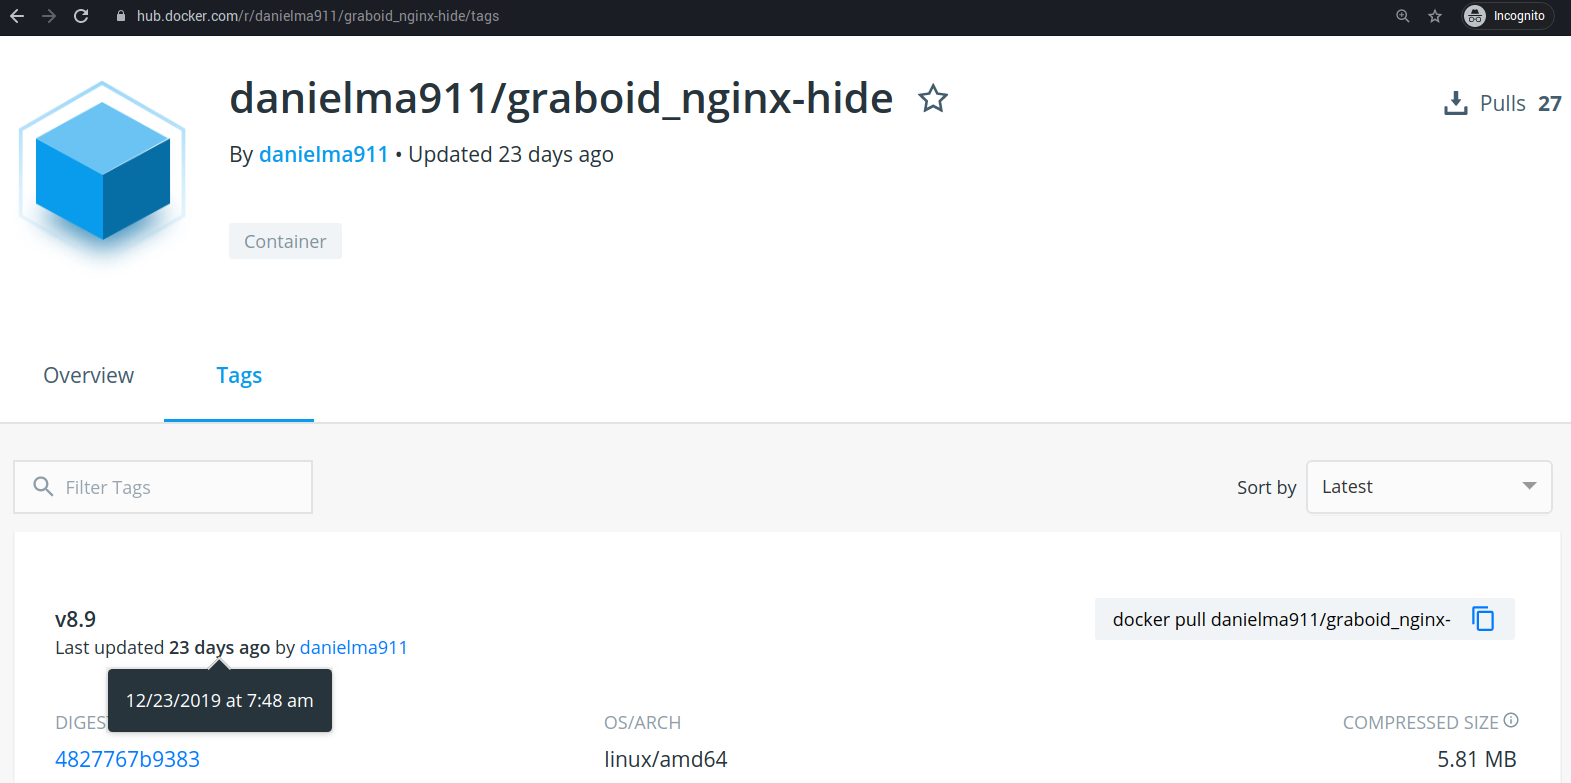
\includegraphics[width=14cm, keepaspectratio]{problema/docker_image_graboid.png}
    \caption*{\textbf{Fuente:} Elaboración propia}
  \end{figure}

  En cuanto al entorno de virtualización Docker, las pruebas se realizaron en la versión 19.03.5-ce, build 633a0ea838.

  El sistema operativo utilizado tanto para el cliente como para el servidor, fue Ubuntu 18.04.3 LTS, corriendo sobre el kernel 5.0.0-32.34, con el entorno gráfico Xfce.

  El navegador web utilizado para las pruebas fue Mozilla Firefox versión 68.0, basado en el motor Gecko versión 20100101.

  Para la captura de paquetes de red se utilizó el software Wireshark versión 3.2.0.

  El análisis contempla la generación de un contenedor con el servicio nginx infectado cuyo acceso fue a través del puerto 80, los procesos iniciados en el cliente mediante la ejecución del script de javascript encargado de la minería de criptomonedas, la medición del rendimiento antes, durante y después de la ejecución del proceso de infección y la captura de paquetes de red generados por la minería.

\end{document}